\documentclass[12pt,titlepage,a4page , tikz , multi,table , svgnames,xcdraw]{article}
\usepackage{graphicx}
\usepackage[svgnames , table , xcdraw]{xcolor} 
\usepackage{fancyhdr}
 
\usepackage{hyperref}
\hypersetup{
    colorlinks=true,
    linkcolor=blue,
    filecolor=magenta,      
    urlcolor=cyan,
}

\usepackage{mathtools}
\usepackage{multirow}
\usepackage{graphicx}
\usepackage{float}
\usepackage{enumitem}
\usepackage{listings }
\usepackage[a4paper, total={6in, 8in}]{geometry}
\usepackage{afterpage}
\usepackage{amssymb}
\usepackage{pdflscape}
\usepackage{lscape}
\usepackage{amsmath}
\usepackage{svg}
\usepackage[final]{pdfpages}

\usepackage{pgf, tikz}
\usetikzlibrary{arrows, automata}
\usetikzlibrary{shapes.multipart}


\usepackage[T1]{fontenc}
\usepackage{tikz}
\usepackage[utf8]{inputenc} % Required for inputting international characters
\usepackage{PTSerif} 

\usepackage{float}

\usepackage[Kashida]{xepersian}
\settextfont[
 BoldFont={XB NiloofarBd.ttf}
 ]{XB Niloofar.ttf}


\NewDocumentCommand{\codeword}{v}{
\texttt{\textcolor{blue}{#1}}
}
\DeclareFixedFont{\ttb}{T1}{txtt}{bx}{n}{12} % for bold
\DeclareFixedFont{\ttm}{T1}{txtt}{m}{n}{12}  % for normal


\definecolor{deepblue}{rgb}{0,0,0.5}
\definecolor{deepred}{rgb}{0.6,0,0}
\definecolor{deepgreen}{rgb}{0,0.5,0}

\newcommand\independent{\protect\mathpalette{\protect\independenT}{\perp}}
\def\independenT#1#2{\mathrel{\rlap{$#1#2$}\mkern2mu{#1#2}}}

% Python style for highlighting
\newcommand\pythonstyle{\lstset{
language=Python,
basicstyle=\ttm,
otherkeywords={self},             % Add keywords here
keywordstyle=\ttb\color{deepblue},
emph={MyClass,__init__},          % Custom highlighting
emphstyle=\ttb\color{deepred},    % Custom highlighting style
stringstyle=\color{deepgreen},
frame=tb,                         % Any extra options here
showstringspaces=false            % 
}}


% Python environment
\lstnewenvironment{python}[1][]
{
\pythonstyle
\lstset{#1}
}
{}

% Python for external files
\newcommand\pythonexternal[2][]{{
\pythonstyle
\lstinputlisting[#1]{#2}}}

\newenvironment{changemargin}[2]{%
\begin{list}{}{%
\setlength{\topsep}{0pt}%
\setlength{\leftmargin}{#1}%
\setlength{\rightmargin}{#2}%
\setlength{\listparindent}{\parindent}%
\setlength{\itemindent}{\parindent}%
\setlength{\parsep}{\parskip}%
}%
\item[]}{\end{list}}

% Python for inline
\newcommand\pythoninline[1]{{\pythonstyle\lstinline!#1!}}


\begin{document}

\begin{titlepage}

 \begin{center}
        
       \vspace*{1cm}

 \vspace{1cm}
       \textbf{ \Huge{به نام خدا} }
       \vspace{0.4cm}
       
       
\includegraphics[width=0.4\textwidth]{sharif1.png}
       
 	\vspace{0.7cm}
       \textbf{ \LARGE{معماری کامپیوتر} }

 
   \vspace{0.7cm}
  \textbf{ \Large{ پروژه پایانی - بخش اول - طراحی پردازنده} }
   \vspace{0.5cm}
       
 
      \large \textbf{دانشکده مهندسی کامپیوتر}\\\vspace{0.2cm}
    \large   دانشگاه صنعتی شریف\\\vspace{0.25cm}
      
استاد:\\
    \textbf{{جناب آقای دکتر اسدی}}

    \vspace{0.15cm}
    \noindent\rule[1ex]{\linewidth}{3pt}
    
    \vspace{0.5cm}
نام، نام خانوادگی و شماره دانشجویی اعضای گروه:\\
    \textbf{{سپهر پورقناد - 97101359}}
        \vspace{0.1cm}
        
     \textbf{{سیدمحمدصادق کشاورزی - 97106249}}
        \vspace{0.1cm}
        
       \textbf{{امیرمهدی نامجو - 97107212}}
        \vspace{0.1cm}


\end{center}
\end{titlepage}

\newpage
\pagestyle{fancy}
\fancyhf{}
\fancyfoot{}

\cfoot{\thepage}
\chead{پروژه پایانی}
\rhead{طراحی پردازنده}
\lhead{معماری کامپیوتر}



\newpage

\section{مقدمه}

هدف اصلی ما در این پروژه، طراحی یک پردازنده ساده بر اساس دستورات داده شده در مستندات آن و تست کردن آن به شکلی بوده است که حالات مختلف آن پوشش داده شود. در طراحی پردازنده داده شده، ما از اصول کلی که در درس آموخته‌ایم و عموماً بر اساس پردازنده مبتنی بر MIPS بوده‌اند، استفاده کرده‌ایم. البته در این جا ساختار کلی ما از لحاظ کلی ساده‌تر از MIPS است. در ادامه گزارش، به توضیح نحوه طراحی بخش‌های مختلف این پردازنده می‌پردازیم.


\newpage

\section{طراحی ALU}

بخش ALU در اصل سیستم محاسبه‌گر اصلی ما است و از آنجایی که بیش‌تر دستورات داده شده در مستندات پروژه برای اجرای به آن وابستگی دارند، از اهمیت بالایی برخوردار است. برای طراحی ALU به این شکل عمل کرده‌ایم پنج ورودی برای آن در نظر گرفته‌ایم که شامل داده ورودی 1، داده ورودی 2 هر دو به صورت 32 بیتی، مقدار شیفت به صورت 5 بیتی، مقدار cin یعنی carry ورودی به صورت 1 بیتی و همچنین Opcode به صورت چهار بیتی بوده است. 

برای عملیات‌های مختلف آن، از ماژول‌هایی که در Quartus در اختیار ما قرار گرفته است، استفاده کرده‌ایم. برای جمع از ماژول جمع کننده استفاده کرده و همچنین از آنجایی که کوارتوس برای آن از سیستم محاسبه Overflow هم پشتیبانی می‌کند، آن را هم قرار داده‌ایم. برای تفریق از ماژول تفریق گر استفاده کرده‌ایم، البته روش‌های دیگری هم نظیر نقیض کردن ورودی دوم و استفاده از cin=1 به عنوان ورودی جمع کننده هم برای این کار وجود داشت ولی برای طراحی ساده‌تر و امکان دیباگ راحت‌تر، ترجیح دادیم که از ماژول جداگانه استفاده کنیم. برای شیفت به چپ و راست، ماژول‌های مربوط به آن‌ها را قرار داده‌ایم. این ماژول‌ها مقدار ShiftAmount را با نام distance و خود داده را هم با عنوان data به عنوان ورودی می‌گیرند. برای NAND یک گیت NAND دو ورودی قرار داده‌ایم که به ورودی‌های آنان، با توجه به این که کوارتوس توانایی تشخیص این که از مقادیر چند بیتی استفاده بکنیم را هم دارد، مقادیر 32 بیتی مربوطه را داده و مقدار 32 بیتی خروجی گرفته‌ایم. برای عملیات \lr{set on less than} از یک ماژول Comparator استفاده کرده‌ایم. این ماژول به عنوان ورودی دو داده 32 بیتی را گرفته و در خروجی دو داده به ما می‌دهد؛ داده aeb در صورتی که $1$ باشد، بیانگر برابر بودن دو مقدار و در غیر این صورت، بیانگر نامساوی بودن آنان است، داده alb هم در صورت یک بودن، نشانگر کوچک‌تر بودن a از b و در غیر این صورت نشان‌دهنده بزرگ‌تر مساوی بودن b از a است. از سیگنال alb برای حالت slt استفاده کرده‌ایم و از آنجایی که این خروجی 1 بیتی است ولی به عنوان خروجی ALU ما 32 بیت می‌خواهیم، سایر بیت‌ها را از طریق اتصال به GND صفر کردیم. در نهایت هم ماژول min را استفاده کرده‌ایم که همان طور که از نامش مشخص است، کمینه دو داده را حساب می‌کند.

برای انتخاب این که خروجی کدام ماژول باید به عنوان خروجی نهایی داده شود، از یک مالتی پلکسر 32 بیتی 8 به 1 استفاده کرده‌ایم که البته حالت $100$ آن استفاده خاصی ندارد. برای خروجی sgn که نشانگر علامت خروجی است، از بیت $31$ مقدار خروجی این مالتی پلکسر استفاده کرده‌ایم. همچنین برای خروجی eq هم از خروجی aeb ماژول Comparator استفاده کرده‌ایم. برای Overflow هم از آنجایی که سؤال گفته فقط برای جمع باید در نظر گرفته شود، گیت‌هایی قرار داده‌ایم که بر اساس OpCode تنها درصورتی که در حالت جمع باشیم، مقدار Overflow ماژول جمع کننده به خروجی برود و در غیر این صورت، $0$ به خروجی برود. یک ماژول به اسم zero هم قرار داده‌ایم که در اصل در پیاده‌سازی داخلی همان comparator است با این تفاوت که یکی از داده‌های آن به شکل درونی صفر شده است و مشخص می‌کند که آیا خروجی نهایی برابر صفر است یا نه.

شکل کلی ماژول ALU در صفحه بعد قرار دارد.




\begin{landscape}

\thispagestyle{empty}

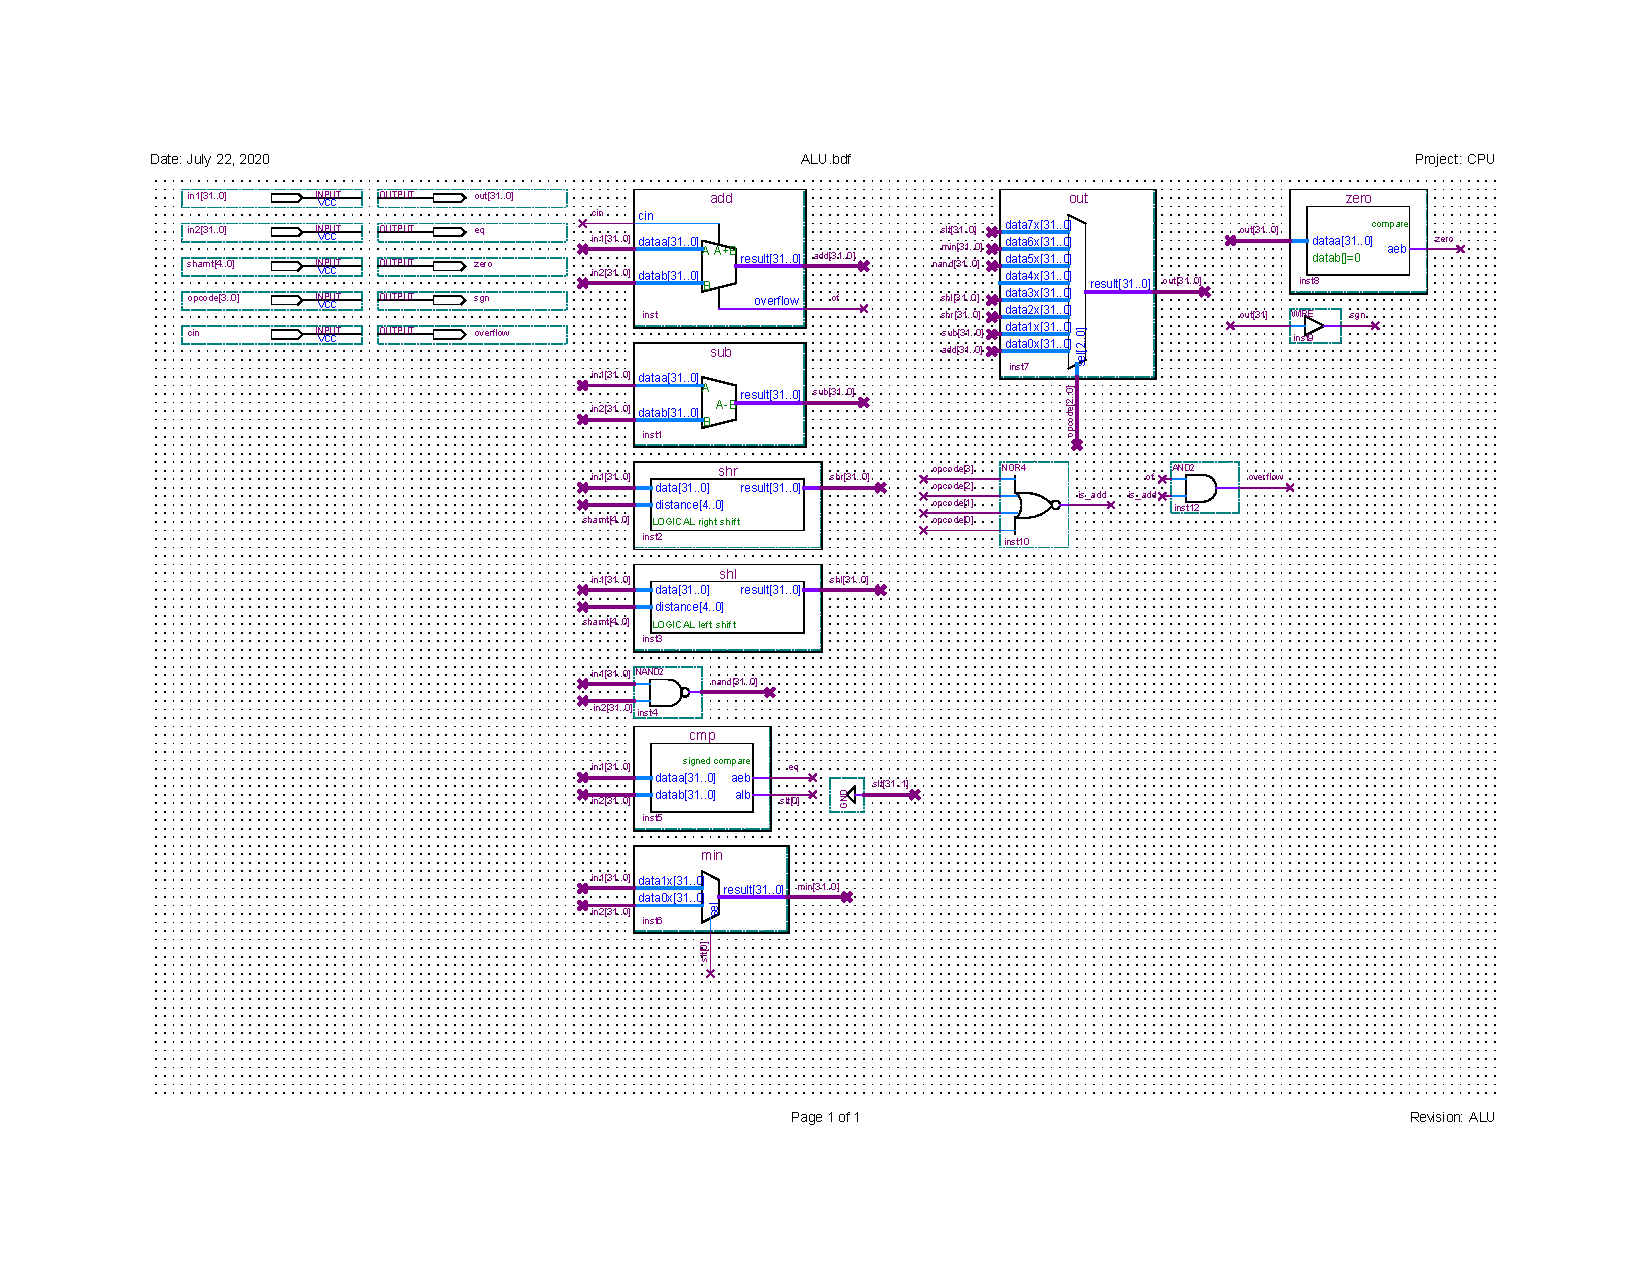
\includepdf[pages=1,angle=90, ]{ALU.pdf}


\end{landscape}




\section{طراحی واحد کنترل}

برای طراحی این پردازنده، ما از 4 کلاک استفاده کرده‌ایم که در شکل زیر \lr{State Machine} آن قرار گرفته است. ضمناً این ماشین حالت را به صورت میلی (Mealy) طراحی کرده‌ایم. یعنی ورودی‌های هر حالت، روی نتیجه آن تأثیر دارند. دلیل این موضوع، متفاوت بودن اجرای دستور لود Shamt با سایر دستورات است. در اصل می‌شد برای این دستور چند حالت متفاوت در نظر گرفت ولی برای ساده‌تر شدن طراحی و کارکرد پردازنده بدون نیاز به پیچیدگی‌های مختلف، چهار استیت هر دو را یکسان طراحی کردیم و در عوض سیستم به صورت میلی است که ورودی OpCode روی خروجی‌های هر استیت تأثیر دارد.




\begin{center}


\begin{latin}
    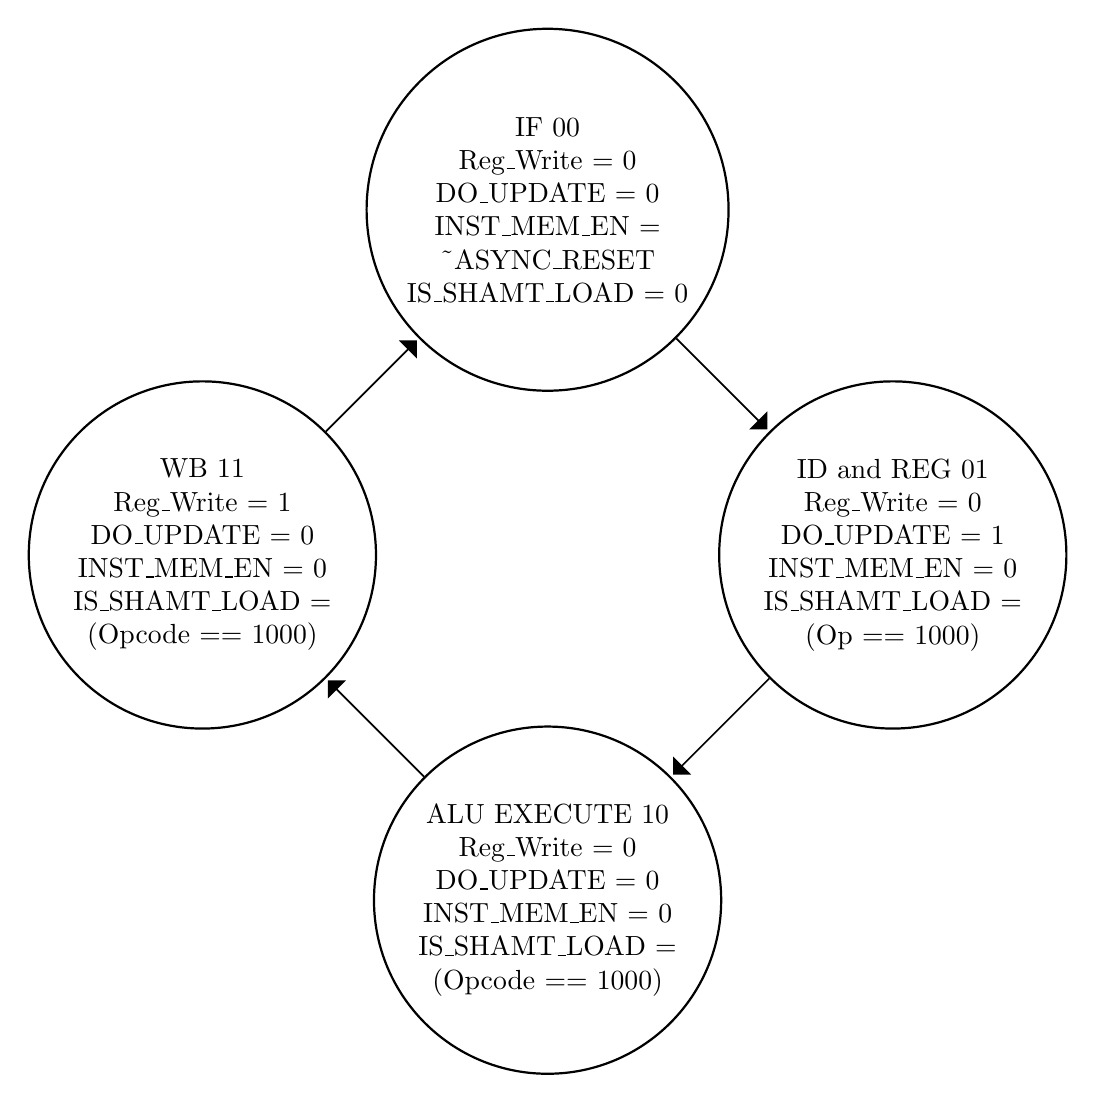
\begin{tikzpicture}[
            > = triangle 90, % arrow head style
            shorten > = 1pt, % don't touch arrow head to node
            auto 
            ,
            node distance = 6.2cm, % distance between nodes
            semithick
            , every text node part/.style={align=center} % line style
        ]

        \tikzstyle{every state}=[
            draw = black,
            thick,
            fill = white,
            minimum size = 4mm
        ]
		
        \node[state] (IF) [] {IF 00  \\ Reg\_Write = 0 \\ DO\_UPDATE = 0 \\ INST\_MEM\_EN =\\ \textasciitilde   ASYNC\_RESET \\ IS\_SHAMT\_LOAD = 0};
        \node[state] (ID) [below right of=IF] {ID and REG 01 \\ Reg\_Write = 0 \\ DO\_UPDATE = 1 \\ INST\_MEM\_EN = 0 \\ IS\_SHAMT\_LOAD =\\ (Op == 1000)};
        \node[state] (EXE) [below left of=ID ] {ALU EXECUTE 10  \\ Reg\_Write = 0 \\ DO\_UPDATE = 0 \\ INST\_MEM\_EN = 0 \\ IS\_SHAMT\_LOAD =\\ (Opcode == 1000)};
        \node[state] (WB) [above left of=EXE] {WB 11 \\ Reg\_Write = 1 \\ DO\_UPDATE = 0 \\ INST\_MEM\_EN = 0 \\ IS\_SHAMT\_LOAD =\\ (Opcode == 1000)};
  






        
		\path[->] (IF) edge node {} (ID);
		\path[->] (ID) edge node {} (EXE);
		\path[->] (EXE) edge node {} (WB);
		\path[->] (WB) edge node {} (IF);
		
       
    \end{tikzpicture}

\end{latin}
\end{center}

\newpage

سیگنال Reg\_Write همان طور که از نام آن مشخص است، مشخص کننده این است که نوشتن روی رجیستر فایل در آن کلاک باید انجام بشود یا خیر. این سیگنال تنها در حالت WriteBack انجام می‌شود.

سیگنال DO\_UPDATE مشخص کننده این است که PC در آن کلاک باید آپدیت بشود یا نه. ما برای اجرای درست دستوراتمان، تنها در حالت $01$ این سیگنال را $1$ می‌کنیم. چگونگی تأثیر این سیگنال را در ادامه و بخش مربوطه، توضیح خواهیم داد.

سیگنال دیگر INST\_MEM\_EN است که در اصل این مشخص می‌کند که \lr{Insturction Register} مقدار جدید را از روی مموری دریافت بکند یا نه. در هر سه استیت $01,10,11$ مقدار آن صفر است و در حالت $IF$ هم اگر سیستم در وضعیت ریست شدن نباشد، مقدار آن $1$ می‌شود و اگر کل سیستم در وضعیت رسیت شدن باشد، مقدار آن صفر است که کلاً \lr{Instruction Register} تغییر نکند.

در نهایت سیگنال IS\_SHAMT\_LOAD مشخص کننده این است که Write\_Data رجیستر فایل باید از خروجی ALU دریافت شود یا بیت 5 تا 14 دستور. در اصل این سیگنال تنها در استیت WB اثرگذار است اما در سه استیت دیگر هم از آن جایی که می‌توان مقدار آن را مشخص کرد، آن را مقداردهی کرده‌ایم. این سیگنال تنها زمانی $1$ می‌شود که OpCode برابر $1000$ یعنی مربوط به دستور \lr{Shamt Load} باشد.


شکل واحد کنترل در صفحه بعد قرار دارد.


\begin{landscape}

\thispagestyle{empty}

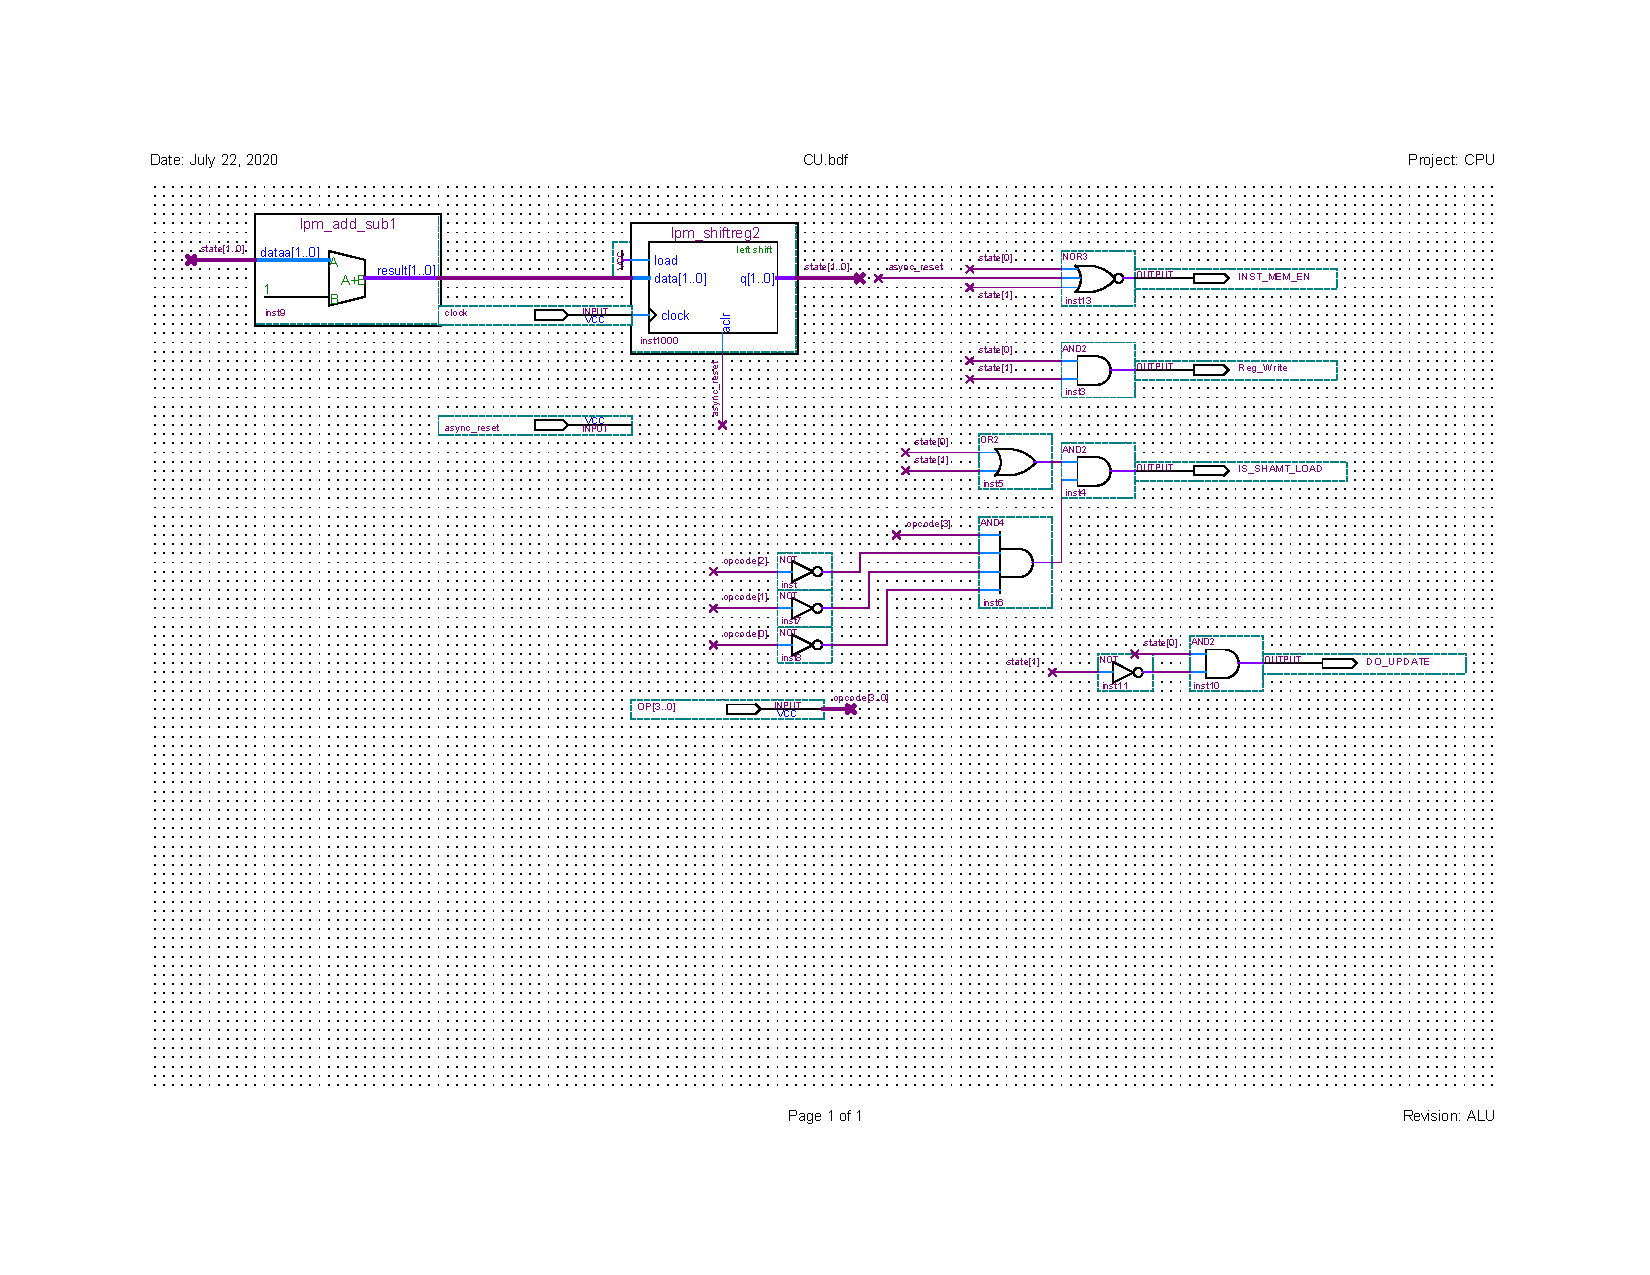
\includepdf[pages=1,angle=90, ]{CU.pdf}


\end{landscape}




\newpage

\section{مقداردهی حافظه دستورات}

برای حافظه دستورات ما از بخش \lr{Mega-Plugin Wizard} ارائه شده توسط Quartus و مقدار دهی ROM بر اساس فایل mif مشابه راهنمای قرار گرفته در مستند پروژه استفاده کرده‌ایم. یکی از نکات قابل توجه این جاست که در CycloneII که تابه‌حال طراحی‌های کوارتوس را با آن انجام دادیم، نمی‌توان رام چندان بزرگی استفاده کرد و مجبور شدیم از رامی با اندازه 32768 کلمه 20 بیتی استفاده کنیم و برای تعداد کلمه بزرگ‌تر، در هنگام کامپایل به خطای در اختیار نبودن منبع برای سنتز چنین چیزی روی CycloneII بر می‌خوردیم.

محتویات فایل mif قرار گرفته بدین صورت است. در جلوی دستورات به صورت کامنت، کاری که دستور انجام می‌دهد هم مشخص شده است:


\begin{latin}
\begin{verbatim}
WIDTH=20;
DEPTH=32768;
ADDRESS_RADIX = UNS;          -- The radix for address values is unsigned
DATA_RADIX = BIN;             -- The radix for data values is Binary
CONTENT                       -- start of (address : data pairs)
BEGIN
0 : 10000000000000100001; -- load shamt r1 <-1
1 : 10000000000000100010; -- load shamt r2 <-1
2 : 10000000000001000011; -- load shamt r3 <-10
3 : 10000000000010000100; -- load shamt r4 <-100
4 : 00110000011111000001; -- r1 = r1 << 30
5 : 00000000000000100001; -- r1 = r0 + r1 (0)
6 : 00000000000001000010; -- r2 = r0 + r2 (0)
7 : 00000000000001100011; -- r3 = r0 + r3 (0)
8 : 00000000000010000100; -- r4 = r0 + r4 (0)
9 : 00000000100001000101; -- r5 = r2 + r2 
10 : 00000000010000100110; -- r6 = r1 + r1 -> must overflow
11 : 00100001000000100100; -- r4 = r4 >> 1
12 : 01010001000001100111; -- r7 = r4 ~& r3
13 : 01110000000010001000; -- r8 = set on less than (r0 , r4)
14 : 01100000100010001001; -- r9 = min(r2 , r4)
15 : 10000000000000101010; -- load shamt r10 <-1
16 : 00010000000101001011; -- r11 = r0 - r10 (answer must be -1)
17 : 01110010110001101100; -- r12 = set on less than (r11 , r3) -> answer = 1
18 : 01100010110000001101; -- r13 = min(r11 , r0) -> answer r11 that is -1
19 : 00000000000000100001; -- r1 = r0 + r1 (0)
20 : 00000000000001000010; -- r2 = r0 + r2 (0)
21 : 00000000000001100011; -- r3 = r0 + r3 (0)
22 : 00000000000001000010; -- r4 = r0 + r4 (0)
23 : 00000000000010100101; -- r5 = r0 + r5 (0)
24 : 00000000000011000110; -- r6 = r0 + r6 (0)
25 : 00000000000011100111; -- r7 = r0 + r7 (0)
26 : 00000000000100001000; -- r8 = r0 + r8 (0)
27 : 00000000000100101001; -- r9 = r0 + r9 (0)
28 : 00001000000101001010; -- r10 = r0 + r10 + cin(1)
29 : 00000000000101101011; -- r11 = r0 + r11
30 : 00000000000101001010; -- r10 = r0 + r10
31 : 00000000000110001100; -- r12 = r0 + r12
32 : 00000000000110101101; -- r13 = r0 + r13 
[33..32767] : 00000000000000000000;
END;


\end{verbatim} 
\end{latin}

نکته مهم در مورد دستورات آخر که اکثراً جمع با صفر هستند، این است که به کمک این دستورات و Output های قرار داده شده، مقادیر هر کدام از رجیسترها را مشاهده بکنیم که ببینیم آیا در نهایت مقادیر قرار گرفته در آنان درست است یا نه.

خروجی‌های نهایی رجیسترها، باید به شکل زیر باشد (یعنی در خط‌های آخر، باید این اعداد را مشاهده کنیم):


\begin{latin}

\begin{verbatim}

R1 = 1073741824
R2 = 1
R3 = 2
R4 = 1
R5 = 2
R6 = -2147483648 -- this is caused by overflow on address 10
R7 = -3
R8 = 1
R9 = 1
R10 = on line 26 it is 1 and then on address 28 it is 2
R11 = -1
R12 = 1 (is -1 less than 2)
R13 = -1 (minimum of -1 and 0)



\end{verbatim}


\end{latin}

ضمناً باید توجه کنیم که این ROM ها به صورت Word-Addressable هستند و از طرفی PC ما چهار واحد چهار واحد جلو می‌رود و همچنین با توجه به فضای داده شده، برای یافتن آدرس درست تنها به 15 بیت نیاز دارند، ما از بیت $2$ تا $16$ PC را به آن به عنوان ورودی آدرس داده‌ایم. دو بیت اول در اصل همیشه $0$ هستند و با توجه به Word-Addressable بودن رام نیازی به آن نیست.



\section{PC و RF}

برای این دو بخش، همان طور که در صورت پروژه خواسته شده بود، از ماژول‌های طراحی شده تمرین 6 و تمرین 7 استفاده شده است. ماژول تمرین 7 عیناً قرار گرفته و ماژول تمرین 6 هم با تغییر کوچکی در مورد Reset مورد استفاده قرار گرفته است. از آن جایی که Reset ای که ما در این جا قرار دادیم، در همه بخش‌ها به صورت \lr{Active High} بود، ریست تمرین 6 که مربوط به PC بود را هم به همین صورت تغییر داده‌ایم.

دو نکته مهم وجود دارد. برای این که در این جا، از مواردی نظیر Jump در PC استفاده نمی‌کنیم و همواره یا PC باید ثابت باشد، یا 4 واحد به جلو برود، از این روش استفاده کردیم که PC را همواره در حالت Branch قرار داده‌ایم. در حالت‌هایی که می‌خواهیم PC ثابت بماند، به عنوان Offset به آن مقدار $-1$ را می‌دهیم که با دو واحد شیفت به چپ درون واحد محاسبه‌گر $PC$ تبدیل به $-4$ می‌شود از آن جایی که در حالت Branch مقدار آن به صورت $PC + 4 + Branch\_Offset$ محاسبه می‌شود، در این حالت، $PC$ ثابت می‌ماند. در زمان‌هایی هم که می‌خواهیم $PC$ به اندازه 4 واحد جلو برود، مقدار $0$ را به عنوان $Offset$ می‌دهیم. این که چه مقداری به $PC$ داده شود، با سیگنال $DO\_UPDATE$ کنترل می‌شود. نکته مهم دیگر هم این است که مقدار ورودی Write\_Data رجیستر فایل از طریق یک مالتی پلکسر با سیگنال کنترلی IS\_SHAMT\_LOAD کنترل می‌شود که در صورتی که $0$ باشد، خروجی $ALU$ مد نظر قرار گرفته و در صورتی که $1$ باشد، مقدار Zero Extend شده بیت‌های 5 تا 15 دستور معیار قرار می‌گیرد.






\section{کنار هم قرار دادن قطعات}

برای کنار هم قرار دادن قطعات استفاده شده، تقریباً از روشی مشابه آن چه که در اسلایدهای درس مشاهده کرده‌ایم استفاده شده است. به این نکته هم توجه شده که در خروجی RF دو عدد فلیپ فلاپ برای ذخیره خروجی آن‌ها و همچنین در خروجی ALU هم یک فلیپ فلاپ دیگر قرار داده‌ایم. در اصل این‌ها معادل همان رجیسترهای اسلایدها هستند که عملاً چون رجیسترهای کوارتوس در این مورد خاص، به جز استفاده از منابع بیش‌تر به خاطر قابلیت شیفت دادن، هیچ مزیتی به فلیپ فلاپ ندارند، مستقیماً از فلیپ فلاپ استفاده کرده‌ایم.

نکته قابل توجه دیگر هم این است که برای شلوغ نشدن یکسری از اتصالات، به جای وصل کردن سیم‌ها به صورت خط روی شکل، از این قابلیت کوارتوس استفاده کرده‌ایم که اگر دو سیم نام مشابهی داشته باشند، اتصال بین آن‌ها را خود کوارتوس تشخیص می‌دهد. بدین ترتیب، به جز برای بخش‌هایی که برای وضوح بیش‌تر شکل لازم بوده، در سایر بخش‌ها از کشیدن سیم‌ها به صورت خط اجتناب کرده‌ایم و از نام‌گذاری‌ها استفاده کرده‌ایم که جلوی شلوغ شدن شکل را می‌گیرد. شکل آن در صفحه بعد قرار دارد.



\begin{landscape}

\thispagestyle{empty}

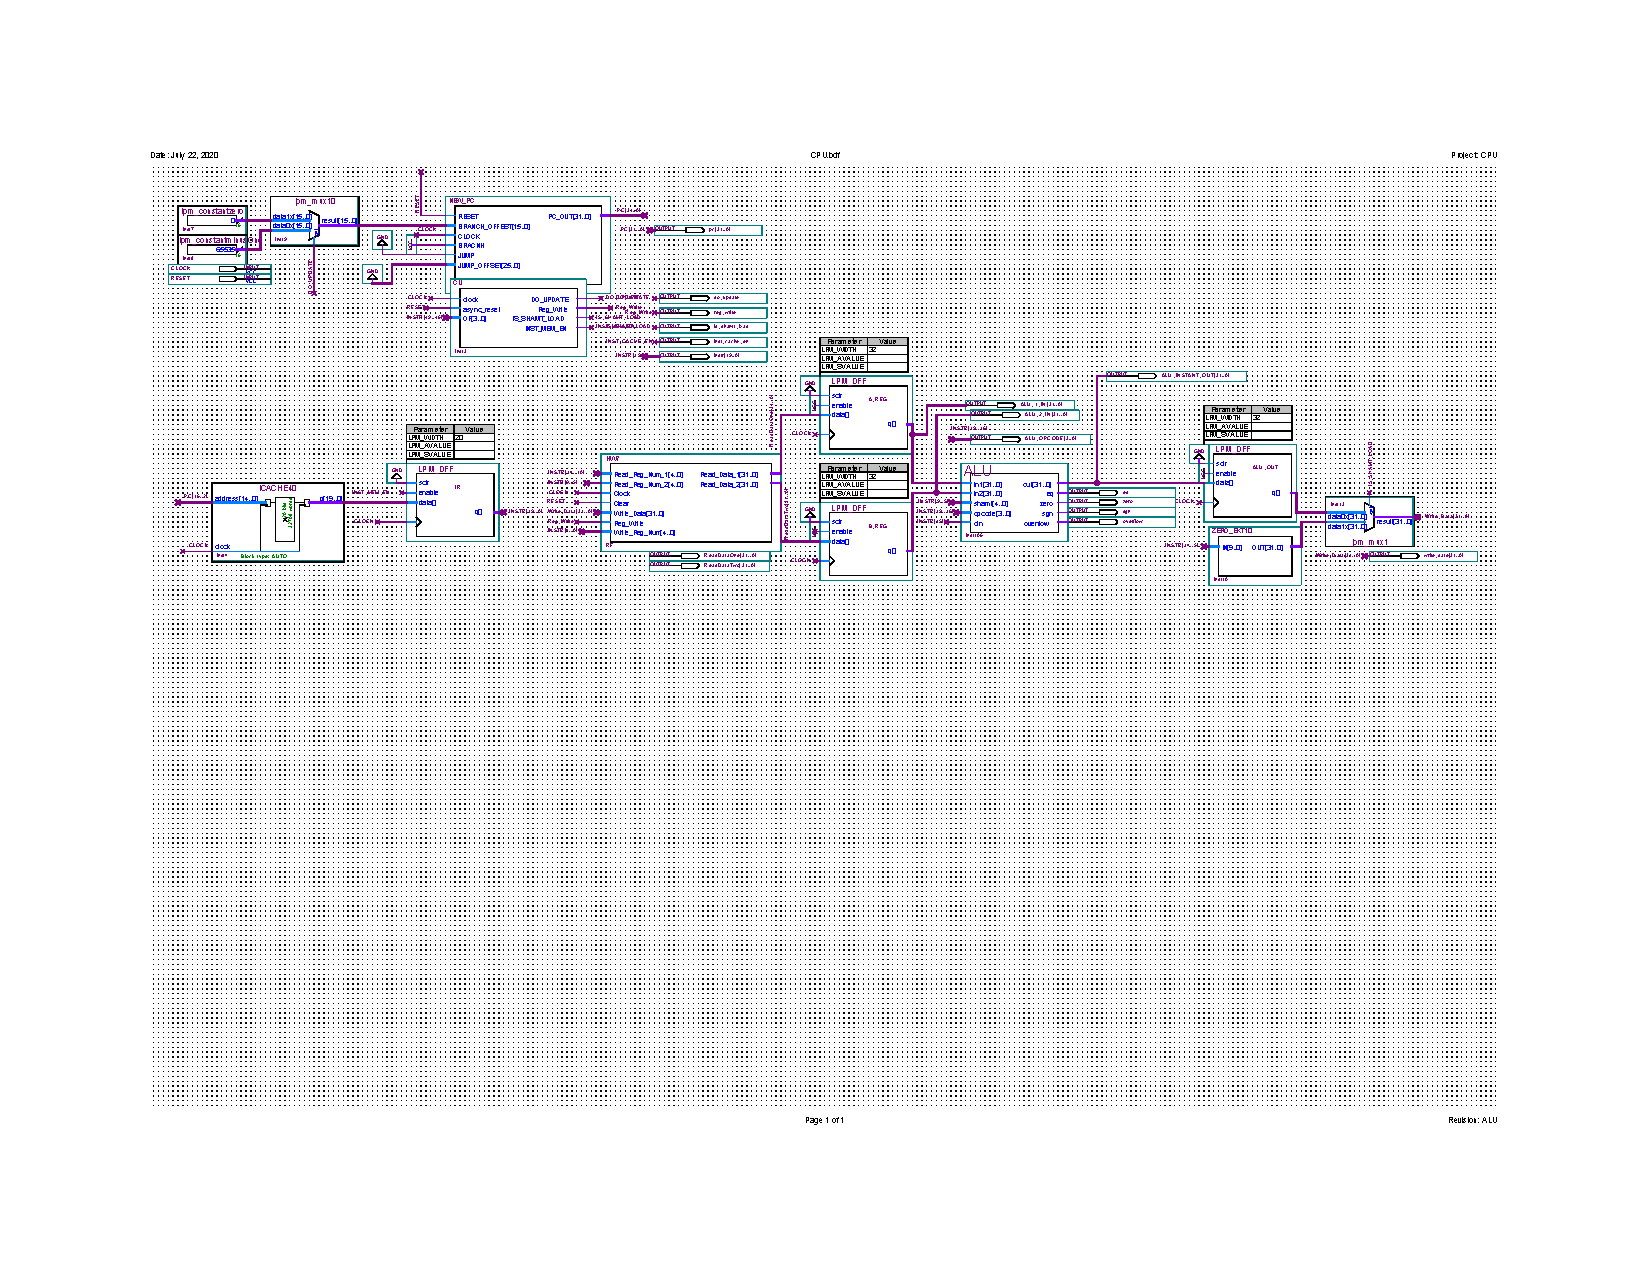
\includepdf[pages=1,angle=90, ]{CPU.pdf}


\end{landscape}

\section{تست پردازنده}

برای تست پردازنده هم، همان دستوراتی که در بخش مقداردهی حافظه دستورات ذکر کردیم را استفاده کردیم. خروجی تمامی سیگنال‌های موردنظر با توجه به موارد گفته شده، درست بوده است. توجه کنید که از بخشی از ویوفرم به بعد، دیگر دستور قابل توجهی نداشتیم و صرفاً جمع کردن $0$ با $0$ بوده است که برای این که حافظه خالی نباشد، قرار داده‌ایم. نکته مهمی که وجود دارد، این است که حتماً باید سه کلاک اول RESET برابر 1 باشد. دلیل این موضوع این است که حافظه دستورات ساخته شده توسط کوارتوس، دو فلیپ فلاپ در ورودی و خروجی خود دارد و سه کلاک طول می‌کشد تا عملکرد آن‌ها به حالت باثبات و پایدار برسد. پس از آن، عملکرد سیستم درست است و برای همین باید سه کلاک اول سیستم در وضعیت RESET باشد. در زیر شکل آن را قرار داده‌ایم. توجه کنید که شکل قابل زوم کردن است. ضمن این که یک فایل ویدیویی هم در کنار گزارش کار قرار دارد که روی تک‌تک کلاک‌ها حرکت می‌کنیم و امکان مشاهده تک‌تک سیگنال‌ها میسر است.

ضمناً لازم به ذکر است که فایل اصلی پروژه \lr{CPU.bdf} و فایل اصلی تست و ویوفرم \lr{CPU2.vwf} نام دارد و بقیه فایل‌ها مربوط به سایر قسمت‌ها و یا ویوفرم های تست ماژول‌های جداگانه هستند.


\begin{center}
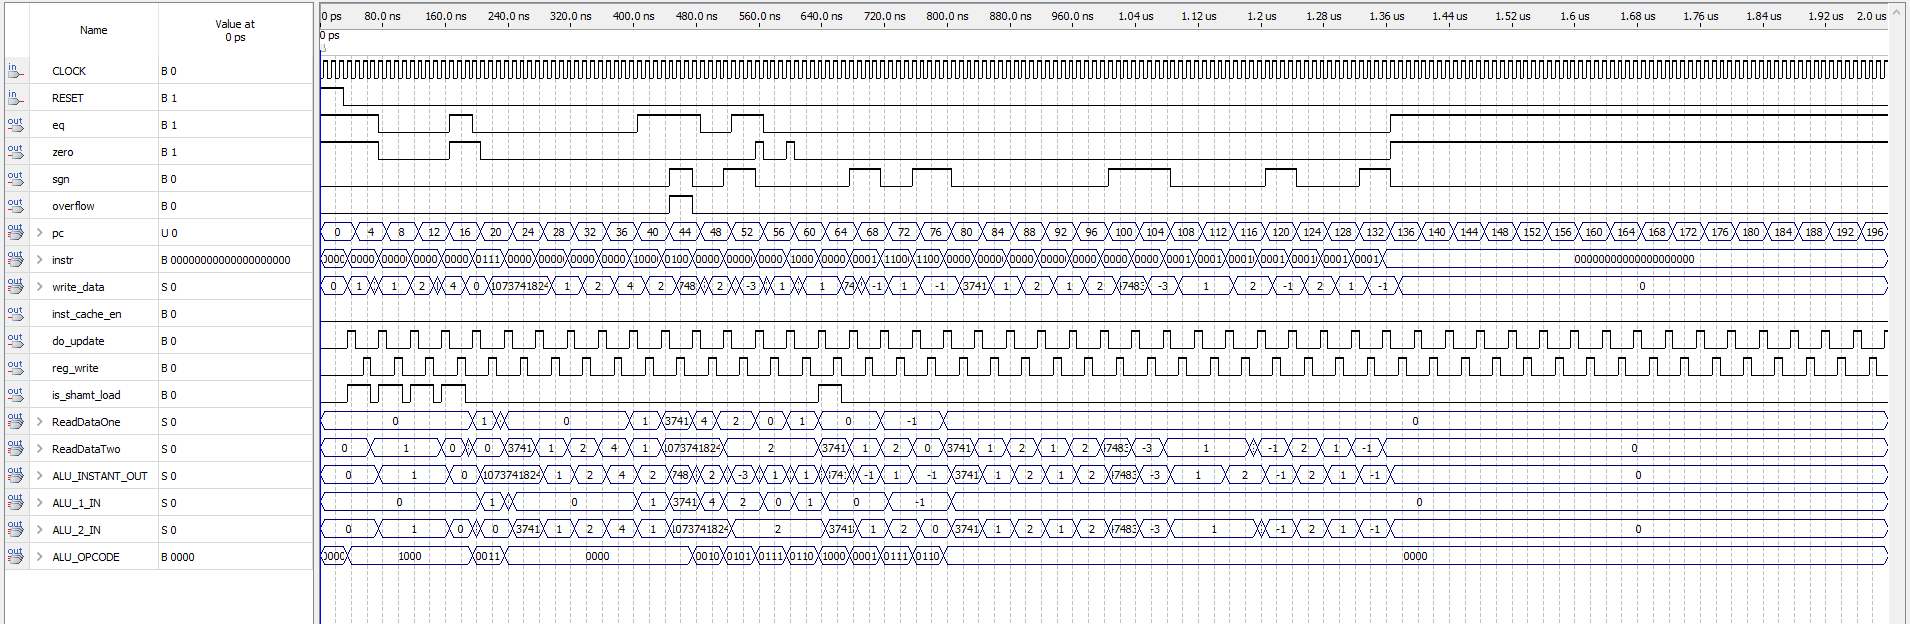
\includegraphics[width=\textwidth]{Waveform.png}
\end{center}




\end{document}












